\documentclass{beamer}

%% docs: https://en.wikibooks.org/wiki/LaTeX/Presentations#Introductory_example

\usetheme{Berlin}
%\usecolortheme{beaver}


%% Title Page

\title{Birdhouse Architecture}
%\subtitle{subtitle}
\author{
Carsten Ehbrecht\\
\medskip
{\scriptsize \url{ehbrecht@dkrz.de}}
}
\institute{German Climate Computing Center (DKRZ)}
\date{October 2015}
\subject{Climate Science, Web Processing Service}

\begin{document}

  \begin{frame}[plain]
    \titlepage
  \end{frame}

  \AtBeginSection[]
  {
    \begin{frame} % shrink
      \frametitle{Outline}
      \tableofcontents[subsectionstyle=hide/hide]
    \end{frame}
  }

  \section{Motivation}

  \begin{frame}
    \frametitle{Web Processing Service}
    A web service interface to standardize the way that algorithms are made available on the Internet
    \begin{figure}
      \includegraphics[width=7cm]{images/Wps.png}
    \end{figure}
  \end{frame}

  \begin{frame}[plain]
    \frametitle{WPS Use Case}
    \begin{figure}
      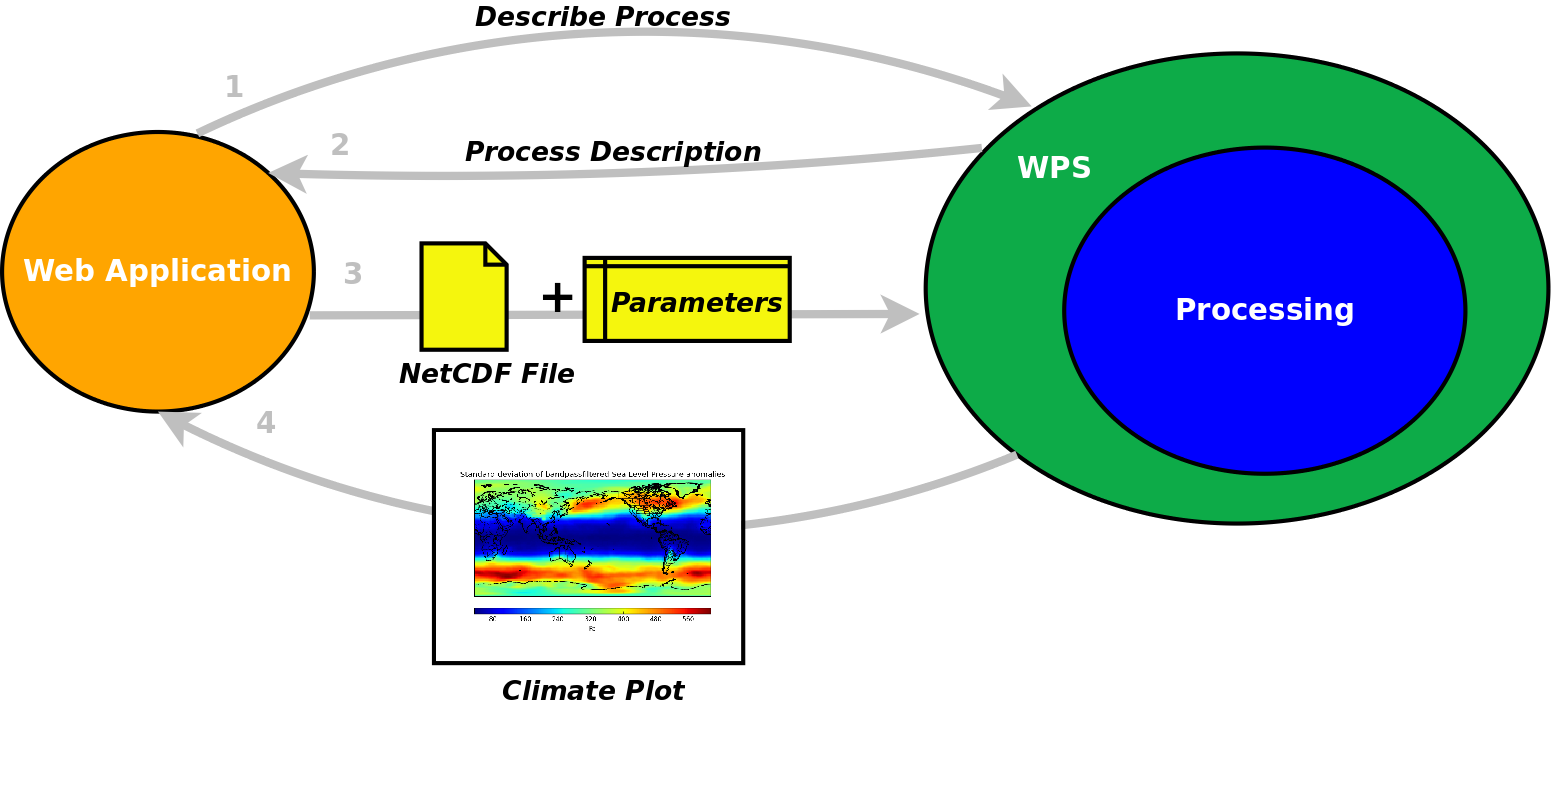
\includegraphics[width=11.5cm]{images/WpsUseCase.png}
    \end{figure}
  \end{frame}

  \begin{frame}[plain]
    \frametitle{Example: Textgenerator + Word Counter}
    \begin{columns}[T] % contents are top vertically aligned
      \begin{column}[T]{5cm} % each column can also be its own environment
        \begin{figure}
          \includegraphics[height=6cm]{images/WpsTextGenerator.png}
        \end{figure}
      \end{column}
      \begin{column}[T]{5cm} % alternative top-align that's better for graphics
        \begin{figure}
          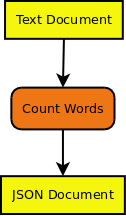
\includegraphics[height=6cm]{images/WpsInOut.png}
        \end{figure}
      \end{column}
    \end{columns}
  \end{frame}

  \begin{frame}[plain]
    \frametitle{Example: WPS Chain}
    \begin{figure}
      \includegraphics[height=6cm]{images/WpsChain.png}
    \end{figure}
  \end{frame}

  \section{Birdhouse Components}

  \begin{frame}
    \frametitle{Birdhouse Components}
     \begin{figure}
       \begin{center}
         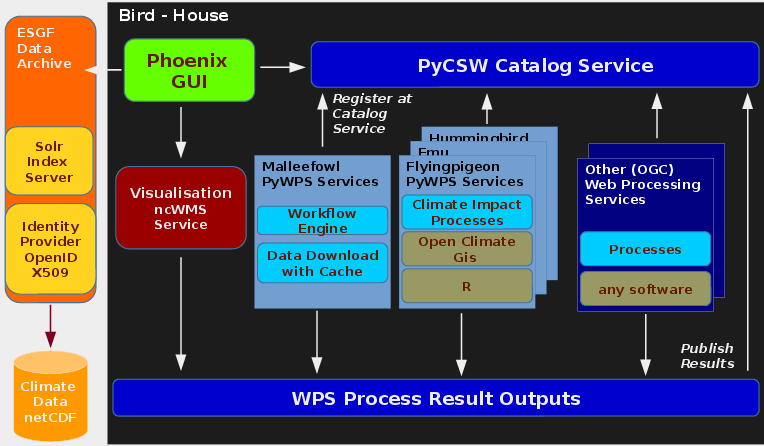
\includegraphics[width=10cm]{images/birdhouse.png}
       \end{center}
    \end{figure}
  \end{frame}

  \begin{frame}
    \frametitle{WSGI Application controlled with Supervisor}
     \begin{figure}
      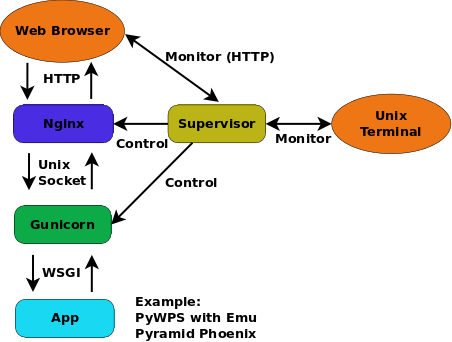
\includegraphics[width=8cm]{images/WsgiApp.png}
    \end{figure}
  \end{frame}

  \section{Birdhouse Builder}

  \begin{frame}
    \frametitle{conda and buildout}
    %Content goes here
  \end{frame}


  \section{Deployment with Docker}

  \begin{frame}
    \frametitle{docker containers and linkage}
    %Content goes here
  \end{frame}


  \section{Security and Interoperability}

  \begin{frame}
    \frametitle{security proxy and best practises to make wps interchangeable}
    %Content goes here
  \end{frame}

  \appendix

  \section{Appendix}
  
   \begin{frame}[allowframebreaks]
    \frametitle<presentation>{Further Reading}    
    \begin{thebibliography}{10}    
      \beamertemplatearticlebibitems
    \bibitem{foos4g-ebrahim}
      Evaluation of WPS Frameworks
      \newblock http://www.slideshare.net/mepa1363/foss4g-ebrahim
    \bibitem{wps-cct}
      Web Processing Service
      \newblock http://www.slideshare.net/GasperiJerome/20130530-web-processing-service-cct-cloud-toulouse-29423710
    \end{thebibliography}
  \end{frame}
  

\end{document}
